\documentclass[tikz, border=5pt]{standalone}
\usepackage{tikz}
\usepackage{amsmath} % For \pi, \frac

\usetikzlibrary{arrows.meta, decorations.markings, patterns.meta, positioning}

\begin{document}
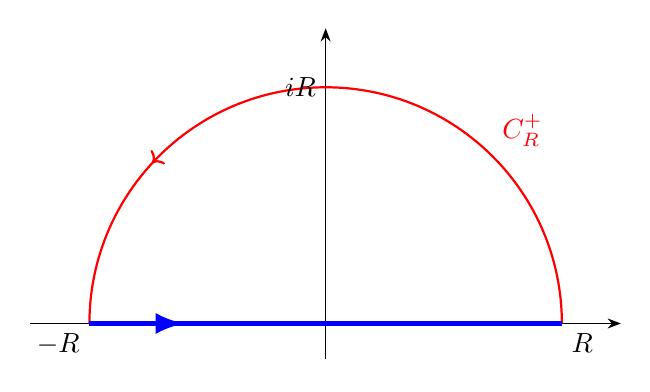
\begin{tikzpicture}[
    scale=1.5, % Adjust scale if needed
    axis/.style={->, >=Stealth, black, thin},
    contour_arc/.style={red, thick},
    contour_line/.style={blue, thick},
    arrow_mark_red/.style={
        decoration={
            markings,
            mark=at position 0.25 with {\arrow{<[red]}} % Arrow on the arc
        },
        postaction={decorate}
    },
    arrow_mark_blue/.style={
        decoration={
            markings,
            mark=at position 0.5 with {\arrow{Triangle[fill=blue, draw=blue, length=3pt, width=5pt]}} % Arrow on the line segment
        },
        postaction={decorate}
    },midarrowL/.style={
        decoration={markings, mark=at position 0.2 with {\arrowreversed{Latex}}},
        postaction={decorate}
    },
    midarrow/.style={
        decoration={markings, mark=at position 0.2 with {\arrow{Latex}}},
        postaction={decorate}
    }
]

% Define Radius
\def\R{2}

% Draw Axes
\draw[axis] (-\R-0.5,0) -- (\R+0.5,0); % x-axis
\draw[axis] (0,-0.3) -- (0,\R+0.5); % y-axis

% Draw Semi-circular Arc (C_R^+)
\draw[contour_arc, arrow_mark_red] (-\R,0) arc (180:0:\R);
\node[red, anchor=south west] at ({cos(45)*\R}, {sin(45)*\R}) {$C_R^+$};

% Draw Line Segment on Real Axis
\draw[contour_line, midarrow, ultra thick] (-\R,0) -- (\R,0);

% Add Labels
\node[black, anchor=north east] at (-\R,0) {$-R$};
\node[black, anchor=north west] at (\R,0) {$R$};
\node[black, anchor=east] at (0,\R) {$iR$};

\end{tikzpicture}
\end{document}